\section{A sharp difference-area inequality for squared bodies}
\label{sec:squared}
Let $\sigma:\mathbb C\to\mathbb C$ be $\sigma(z)=z^2$. We prove
\[
 \area(\sigma K-\sigma K)\leq5\area(\sigma K)
\]
for every origin-symmetric planar convex body $K$, with a sharp constant.
The proof identifies squared bodies with planar reciprocal bodies, reduces
arbitrary sources to parallelograms, and bounds their squares by a geometric
argument valid in every dimension. The last argument gives a sharp
supremum for intersections of two confocal paraboloids; it does not bound
arbitrary higher-dimensional reciprocal bodies.

For a planar body $L$ write
\[
 R(L)=\frac{\area(L-L)}{4\area(L)}.
\]
This quotient is invariant under invertible affine maps. The planar bound
is $R\leq5/4$. Through the quaternionic construction of
Chaidez--Tanny~\cite{CT2026}, it bounds $c_{\EHZ}(X)^2$ by
$(5/2)\Vol_4(X)$ for bodies with right quaternionic $I$-symmetry.
We give the Finsler and capacity normalizations at the end of the section.
A \emph{source body} below is compact, origin-symmetric, convex, and has
nonempty interior.

\subsection{Complex squaring and reciprocal convexity}
Following Milman--Milman--Rotem~\cite{MMR2018}, write
\[
 M'=\{y:\langle y,n\rangle\leq h_M(n)^{-1}\ \text{for all }n\in S^1\}.
\]
Their Lemma 18 and Proposition 19 express $M'$ as the intersection, over $x\in M$, of the parabolic regions
\[
 P_x=\{y:\langle y,x\rangle\leq 1-\tfrac14|x|^2|\operatorname{proj}_{x^\perp}y|^2\},\quad P_0=\mathbb R^2.
\]
For $x=re^{i\theta}$, elementary squaring gives
\[
 P_x=\sigma(S_x),\qquad S_x=\{z:|\operatorname{Re}(e^{-i\theta/2}z)|\leq r^{-1/2}\}.
\]
Indeed, in coordinates $e^{-i\theta}y=u+iv$, both descriptions are $u\leq r^{-1}-rv^2/4$. The map $\sigma$ commutes with arbitrary intersections of centrally symmetric sets: the two square roots of a point either both belong to any such set or both fail to belong.

\begin{theorem}[Squared bodies and reciprocity]
The compact planar reciprocal bodies containing the origin in their interior are precisely the images $\sigma(K)$ of source bodies. Moreover,
\[
 (\sigma K)'=\sigma(K^\circ).
\]
\end{theorem}
\begin{proof}
Write $K$ as the intersection of its symmetric supporting strips with unit normals $n=e^{i\phi}$ and half-widths $h_K(n)$. Each strip maps to $P_{x_\phi}$, where $x_\phi=e^{2i\phi}/h_K(n)^2$. Consequently $\sigma K$ is convex. Since $n/h_K(n)$ runs over $\partial K^\circ$, the points $x_\phi$ run over $\partial\sigma(K^\circ)$. This last image is also convex by the same strip argument. The parabolic representation therefore gives
\[
 \sigma K=(\sigma(K^\circ))'.
\]
Apply the same identity to $K^\circ$ to obtain the stated conjugacy. Conversely, the parabolic representation of any reciprocal $M'$ identifies it with $\sigma(\bigcap_{x\in M}S_x)$. The intersection is centrally symmetric and convex; compactness and interior of its square imply the corresponding properties of the intersection itself.
\end{proof}
This is an identity in fixed Euclidean coordinates. Neither squaring nor reciprocity is asserted to commute with arbitrary affine maps.

\subsection{Two confocal paraboloids in arbitrary dimension}

We first record the shadow-system fact used twice below. If points move
parallel to a fixed vector $e$ according to
\[
 C_t=\conv\{p+t\beta(p)e:p\in S\},
\]
then $\Vol_d(C_t)$ is convex in $t$. Indeed, the projection onto
$e^\perp$ is fixed. On each line parallel to $e$, the upper endpoint is
a supremum of affine functions of $t$, and the lower endpoint an infimum:
the admissible convex combinations are specified by their fixed transverse
coordinate. The fiber length is therefore convex, and integration proves
the assertion. If convex bodies $C_t$ are given by such moving points,
then $C_t-C_t$ is another shadow system, with generators $p-q$ and
velocities $\beta(p)-\beta(q)$.

\begin{theorem}[Two-paraboloid difference-volume bound]
\label{thm:two-paraboloids}
Let $d\geq2$, and let $Q\subset\mathbb R^d$ be a bounded intersection
of two solid paraboloids of revolution with a common focus. Then
\[
 \frac{\Vol_d(Q-Q)}{\Vol_d(Q)}<C_d,
 \qquad C_d=\frac{2^{d+1}(d-1)+2}{d}.
\]
The constant $C_d$ is the supremum over this class, and is approached by
an affine-normalized degeneration to the round parabolic cap
\[
 P_d=\{(u,z):0\leq u\leq1,\ |z|^2\leq u\}.
\]
\end{theorem}
\begin{proof}
\emph{Normalize the pair.}
Translate the common focus to the origin. The two inequalities are
\[
 |y|+a_i\cdot y\leq c_i,\qquad |a_i|=1,\quad c_i>0,
 \quad a_1\ne a_2.
\]
The last condition is necessary for boundedness. On the future light cone
$r=|y|$, the covectors $\ell_i=(1,a_i)/c_i$ are null for the quadratic
form $r^2-|y|^2$. Their sum is timelike, since
\[
 (\ell_1+\ell_2)_0^2-| (\ell_1+\ell_2)_{\mathrm{sp}}|^2
 =\frac{2(1-a_1\cdot a_2)}{c_1c_2}>0.
\]
A Lorentz transformation sends that sum to the time axis. The transformed
null covectors then have opposite spatial parts and equal positive time
coordinates. A common rescaling and a spatial rotation give the lens
\[
 L=\{(x,z):\sqrt{x^2+|z|^2}+|x|\leq1\}
   =\{(x,z):|x|\leq\tfrac12,\ |z|^2\leq1-2|x|\}.
\]
This change preserves the class: Lorentz maps preserve the future cone
and future null covectors, so each inequality remains a confocal
paraboloid inequality after division by its positive time coefficient.
A Lorentz transformation is a spatial rotation composed with a boost;
the latter has spatial part
$(y_1,y_\perp)\mapsto(\gamma(y_1+t|y|),y_\perp)$,
where $|t|<1$ and $\gamma=(1-t^2)^{-1/2}$.
Consequently, up to an invertible spatial linear map, every original
$Q$ is
\[
 T_v(L),\qquad T_v(y)=y+|y|v,\quad |v|<1.
\]
These images are convex by the same Lorentz calculation, and remain
convex for $|v|=1$ by Hausdorff continuity.

\emph{Enlarge the shadow family.}
Write $v=ca+b$, where $a$ is the $x$-axis and $b\perp a$. Define
\[
 F_{c,b}(x,z)=(x,z)-|x|(c,b).
\]
We claim that $F_{c,b}(L)$ is convex throughout the larger parameter set
$|c|\leq1$, $|b|\leq1$. For $|c|<1$, its positive and negative halves
are affine images of the half-lenses, on opposite sides of the common
interface $D=\{0\}\times B^{d-1}$. Take one point in either half:
\[
 Y_+=((1-c)t,z-tb),\qquad
 Y_-=(-(1+c)r,w-rb),
\]
where $t,r\geq0$, $|z|^2\leq1-2t$ and $|w|^2\leq1-2r$.
The segment crosses the interface at a point with transverse coordinate
\[
 z_0=\lambda z+(1-\lambda)w-[\lambda t+(1-\lambda)r]b
\]
for some $\lambda\in[0,1]$. Since
$\sqrt{1-2t}\leq1-t$ and likewise for $r$, we have $|z_0|\leq1$.
The crossing lies in $D$, so the whole segment lies in the union of the
two convex halves. This proves convexity; the endpoint values of $c$
follow by continuity.

On $\partial L$ we have $|y|=1-|x|$, and hence
$T_v(y)=v+F_{c,b}(y)$. For $|v|<1$, the map $T_v$ is a homeomorphism:
on each preserved transverse line, its coordinate along $v$ is strictly
increasing. Thus support maxima of $T_v(L)$ occur on $T_v(\partial L)$.
Support maxima of $F_{c,b}(L)$ occur on the two outer parabolic sheets
or the interface rim, also images of points of $\partial L$.
Equality of support functions gives
\[
 T_v(L)=v+F_{c,b}(L),\qquad |v|\leq1,
\]
with the unit-vector case obtained by continuity. This is equality of
image bodies; the maps need not agree at interior points.

The two affine half-maps have determinants $1-c$ and $1+c$.
Their interiors are disjoint and the original half-volumes equal, so
\[
 \Vol_d(F_{c,b}(L))=\Vol_d(L).
\]
For fixed $b$, varying $c$ moves all points parallel to $a$, with speed
$-|x|$. The difference-body volume is therefore convex in $c$, and its
quotient by volume is bounded by the larger quotient at $c=\pm1$.

\emph{Identify the endpoints.}
At $c=1$ the positive half collapses into $D$, because
$|z-tb|\leq|z|+t\leq1$. The negative half has coordinates
\[
 u=-2r,\qquad w=z-rb,\qquad |z|^2\leq1-2r.
\]
The affine change $U=1+u$, $Z=w-(u/2)b$ identifies it with $P_d$.
The other endpoint is its reflection. Writing $\omega_{d-1}$ for the
volume of the unit $(d-1)$-ball, we obtain
\[
 \Vol_d(P_d)=\frac{2\omega_{d-1}}{d+1},\qquad
 \Vol_d(P_d-P_d)=2\omega_{d-1}
   \int_0^1(1+\sqrt{1-s})^{d-1}\,ds.
\]
For fixed difference coordinate $s\geq0$, the transverse difference
balls increase as the source coordinate increases; the largest is
attained at the pair $1,1-s$. Evaluating the integral gives the stated
quotient $C_d$.

Finally, along the original radial shadow $T_{te}(L)$ the volume is
constant: its Jacobian is $1+t\langle e,y\rangle/|y|$, and the odd term
integrates to zero. The quotient at $t=0$ is $2^d<C_d$, whereas that at
$t=1$ is at most $C_d$. Convexity of the numerator gives strictness for
$|t|<1$. As $v\to a$, the images tend to a translate of $P_d$; volume
continuity proves sharpness of the supremum.
\end{proof}

\subsection{Endpoint caps and positive tent decompositions}
For a squared planar body $L$, let
\[
 T_t(u,v)=(u+t\sqrt{u^2+v^2},v),\qquad -1\leq t\leq1.
\]
For $|t|<1$, this is affine equivalent to another squared body, since
\[
 \sigma(\sqrt{1+t}\,x+i\sqrt{1-t}\,y)
 =\bigl(\operatorname{Re}\sigma z+t|\sigma z|,
         \sqrt{1-t^2}\operatorname{Im}\sigma z\bigr).
\]
The images are convex, including the endpoints by continuity. The
Jacobian gives
\[
 \area(T_tL)=A+tB,\qquad A=\area(L),\quad
 B=\int_L\frac{u}{\sqrt{u^2+v^2}}\,du\,dv,
 \qquad |B|<A.
\]
The difference bodies form a shadow system, so their areas are convex
in $t$. Dividing the endpoint interpolation by the positive affine
function $4(A+tB)$ proves
\[
 R(L)\leq\max\{R(T_{-1}L),R(T_1L)\}.
\]
Since $T_1(\sigma(x+iy))=(2x^2,2xy)$, it suffices to bound the caps
\[
 C_K=\{(x^2,xy):(x,y)\in K\}.
\]
The other endpoint is the same construction after exchanging source
coordinates.

Normalize the horizontal projection of $K$ to $[-1,1]$ and write
\[
 K=\{(x,y):-1\leq x\leq1,\ -b(-x)\leq y\leq b(x)\},
\]
where $b$ is concave. A source shear $y\mapsto y+cx$ induces the affine
cap shear $(u,v)\mapsto(u,v+cu)$. Choose it so that
$b(-1)=b(1)=d\geq0$; then $b\geq d$. The cap sections are
\[
 -V_b(u)\leq v\leq U_b(u),\quad
 U_b(u)=\sqrt u\,b(\sqrt u),\quad
 V_b(u)=\sqrt u\,b(-\sqrt u),\qquad 0\leq u\leq1.
\]
Their area $A(b)=\int_0^1(U_b+V_b)$ is linear in $b$. Define
\[
 \begin{aligned}
 H_+(b,s)&=\max_{0\leq u\leq1-s}
               [U_b(u+s)+V_b(u)],\\
 H_-(b,s)&=\max_{0\leq u\leq1-s}
               [V_b(u+s)+U_b(u)].
 \end{aligned}
\]
The upper and lower endpoints of each difference section give
\[
 N(b):=\area(C_b-C_b)
      =2\int_0^1[H_+(b,s)+H_-(b,s)]\,ds.
\]
Each maximum is positively homogeneous and convex in $b$; thus $N$ is
subadditive.

For $-1<a<1$, let
\[
 f_a(x)=\begin{cases}
 (1+x)/(1+a),&x\leq a,\\
 (1-x)/(1-a),&x\geq a.
 \end{cases}
\]
Every continuous concave profile with equal endpoints is a uniform limit
of positive combinations of $1$ and these tents. For piecewise-linear
profiles this follows by matching their slope jumps; uniform concave
piecewise-linear approximation gives the general case. By linearity of
$A$ and subadditivity of $N$, it therefore suffices to prove $N\leq5A$
for the constant profile and for each single tent.

\begin{figure}[tb]
 \centering
 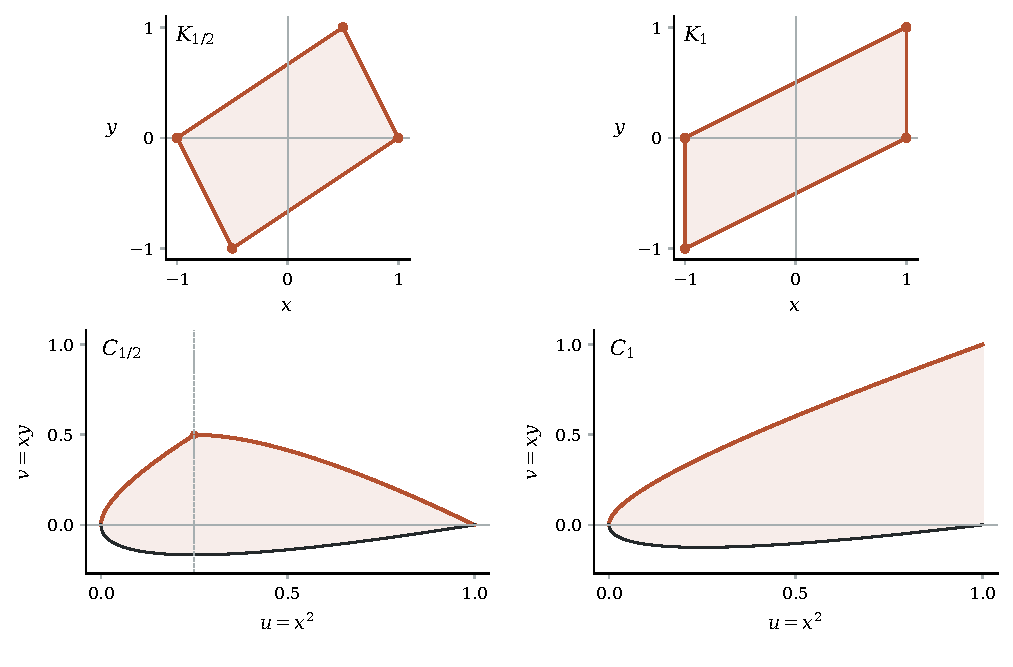
\includegraphics[width=.90\linewidth]{figures/tent-caps-compact.pdf}
 \caption{A single-tent source is a parallelogram. Its cap is a limit of
 affine-normalized squares of flattened parallelograms, so the
 two-paraboloid theorem applies without evaluating the difference-area
 integral.}
 \label{fig:tent-caps}
\end{figure}

\begin{theorem}[Sharp planar difference-area bound]
\label{thm:squared-five}
For every origin-symmetric planar convex body $K$,
\[
 \area(\sigma K-\sigma K)\leq5\area(\sigma K).
\]
The constant five cannot be decreased. The same inequality holds for
all planar reciprocal bodies and their affine images.
\end{theorem}
\begin{proof}
The source of $f_a$ is the parallelogram
\[
 K_a=\conv\{(-1,0),(a,1),(1,0),(-a,-1)\};
\]
the constant profile has a rectangular source. Each is an intersection
of two symmetric strips, so its square is the intersection of two solid
confocal parabolas. Any invertible flattening remains a parallelogram.
Theorem~\ref{thm:two-paraboloids} with $d=2$ bounds the difference-area
quotient of each flattened square by five. After affine normalization,
these squares tend to the corresponding cap; positive limiting area and
Hausdorff continuity pass the bound to that cap. The positive-profile
reduction and then the endpoint reduction prove the inequality.

For sharpness, take $K_\epsilon=[-1,1]\times[-\epsilon,\epsilon]$.
Under $(u,v)\mapsto(u,v/(2\epsilon))$, its square tends to
$P_2=\{0\leq u\leq1,\ |v|\leq\sqrt u\}$, whose difference area is
five times its area. Reciprocity and affine invariance give the remaining
statements. Lower-dimensional sources follow by approximation.
\end{proof}

\subsection{Finsler and symplectic consequences}

We give the normalization in the transfer explicitly. For a Finsler metric
$F$ on $\mathbb{RP}^2$, let $\ell(F)$ be its shortest noncontractible
closed-geodesic length, and put
\[
 \mathcal V(F)=\int_{D_F^*\mathbb{RP}^2}\frac{\omega_{\mathrm{can}}^2}{2}.
\]
This is the unnormalized cotangent volume used by Chaidez--Tanny; it is
$\pi$ times the usual normalized Holmes--Thompson area. Let
$\overline F(v)=(F(v)+F(-v))/2$. Its unit codisks are
$(D_x^*F-D_x^*F)/2$, because the support function of this Minkowski average
is the average of the two tangent norms. The sharp planar theorem therefore gives
\[
 \mathcal V(\overline F)\leq\frac54\mathcal V(F)
\]
whenever all the unit codisks of $F$ are affine images of squared bodies.

\begin{corollary}\label{cor:squared-finsler}
For such a Finsler metric on $\mathbb{RP}^2$,
\[
 \ell(F)^2\leq\frac58\mathcal V(F).
\]
\end{corollary}
\begin{proof}
For any noncontractible loop, at least one of its two orientations has
$F$-length at most its $\overline F$-length. Thus
$\ell(F)\leq\ell(\overline F)$. The reversible Ivanov--Pu inequality,
in the normalization above, is
$\ell(\overline F)^2\leq\mathcal V(\overline F)/2$;
see \cite[Theorem~3.7 and Lemma~3.8]{CT2026}. Combine these inequalities.
\end{proof}

\begin{corollary}\label{cor:I-symmetric}
Let $X\subset\mathbb H$ be a full-dimensional convex body invariant
under right multiplication by the quaternion $I$, with the standard
symplectic structure in \cite{CT2026}. Then
\[
 c_{\EHZ}(X)^2\leq\frac52\Vol_4(X),\qquad
 \rho(X)\leq\frac54.
\]
\end{corollary}
\begin{proof}
First suppose $X$ is smooth and uniformly convex. The quaternionic
construction of Chaidez--Tanny associates a Finsler metric $F$ on
$\mathbb{RP}^2$ whose unit codisks are affine squared bodies. Their
four-sheet contact covering gives
\[
 c_{\EHZ}(X)\leq4\ell(F),\qquad
 \Vol_4(X)=4\mathcal V(F)
\]
(\cite[Theorem~4.4 and equations~(5.2)--(5.3)]{CT2026}). Hence
\[
 c_{\EHZ}(X)^2\leq16\ell(F)^2
 \leq10\mathcal V(F)=\frac52\Vol_4(X).
\]
For arbitrary convex $X$, use smooth uniformly convex approximants with
the same finite symmetry. One obtains them by smoothing the invariant
support function and adding a small Euclidean ball. Hausdorff continuity
of volume and of EHZ capacity passes the bound to $X$, as in
\cite[Remark~5.4]{CT2026}.
\end{proof}

The planar constant five is sharp; neither corollary asserts a sharp
constant for its geometric class. In particular the comparison between a
geodesic and its closed lift, and the compatibility of codisks coming from
one ambient body, may prevent simultaneous equality in the auxiliary
estimates. The corollary gives the explicit constant $\sqrt5/2$ in a setting where
\cite[Theorem~11]{CT2026} supplies an unspecified constant below $\sqrt{3/2}$ ; it does not
establish the Viterbo bound $\rho\leq1$ for $I$-invariant bodies.
